\graphicspath{{chapters/contents/sessio_02/images/}}

\section{Sessió 02 (21/09/26). Física per tot arreu }

\textit{
La física (i la química, com veurem ben aviat) són per tot arreu. Les podem trobar en gairebé qualsevol cosa que ens envolta, i entendre-les una mica millor ens ajuda a comprendre per què passen les coses, prendre decisions amb més criteri i comprendre el món amb molt més coneixement.
}

\textit{
La setmana passada vam veure les diferents branques de la física i la química. Ara n’agafarem només una part molt petita de tot el que podem arribar a estudiar: l’òptica. Buscarem al nostre voltant exemples quotidians on apareguin fenòmens relacionats amb la llum. I podríem fer exactament el mateix amb la calor, l’electricitat, l’oxigen, el sabor dels gelats o gairebé qualsevol altre tema.
}

\section{Nivell I }

La llum és un fenomen bastant més complicat del que sembla. La podem estudiar de moltes maneres: com es genera, com es propaga, com interactua amb la matèria o com transporta energia.

I, mentrestant, és al nostre voltant tot el temps: ajuda les plantes a créixer, regula els nostres ritmes biològics i recorda al teu cos que al matí toca aixecar-se per anar al cole i que a la nit potser ja va sent hora de deixar els reels 'monos' de TikTok i anar a dormir.

La branca clàssica de la física que estudia la llum és \textbf{l’òptica}. Estudia com es propaga, com rebota a les superfícies, com es desvia quan travessa materials i com forma imatges.

Una branca més moderna és la \textbf{fotònica}, que entra en joc sobretot quan volem combinar la llum amb l’electrònica i fer-ne coses útils: làsers, fibra òptica, sensors, comunicacions, plaques solars...

Segur que et sonen alguns experiments d’òptica de tota la vida: la canyeta que sembla trencada dins d’un got d’aigua, un prisma que separa la llum en colors, una moneda que reapareix al fons d’una tassa, una lupa que concentra la llum o una cullera que et torna la cara del revés.

Bé. Intentarem anar una mica més enllà. I si no coneixes aquests experiments, ja tens feina per quan arribis a casa.

\subsection{De veritat viatja en línia recta?}

La llum viatja a una velocitat enorme: aproximadament uns 300.000 km per segon en el buit.
En un segon podria donar unes set voltes i mitja a la Terra. Si encenguessis una llanterna apuntant cap a la Lluna, la llum hi arribaria en poc més d’un segon. Naturalment, això no vol dir que algú a la Lluna veiés la teva llanterna, que ja seria demanar-li massa.


Una paraula que ens farà servei: \textbf{homogeni}. Dit d’una manera intuïtiva: si n’agaféssim un tros petit, aquest tros es comportaria igual que el conjunt. No hi trobaríem una zona que, de cop, tingués propietats diferents de la resta. Vaja, que una galeta amb trossets de xocolata no és precisament un medi homogeni. Una mescla d’aigua amb trossets de gel és un medi transparent però no homogeni.

Quan la llum viatja per un medi transparent i homogeni i ningú no la molesta, pot ser una paret, una mà o el típic senyor alt assegut davant teu al cinema, segueix una trajectòria recta.

Són transparents l’aire, l’aigua, molts líquids, el vidre i, sobretot, el buit.

\subsection{Un raig de llum es troba amb un altre material?}

\begin{figure}[H]
    \centering
    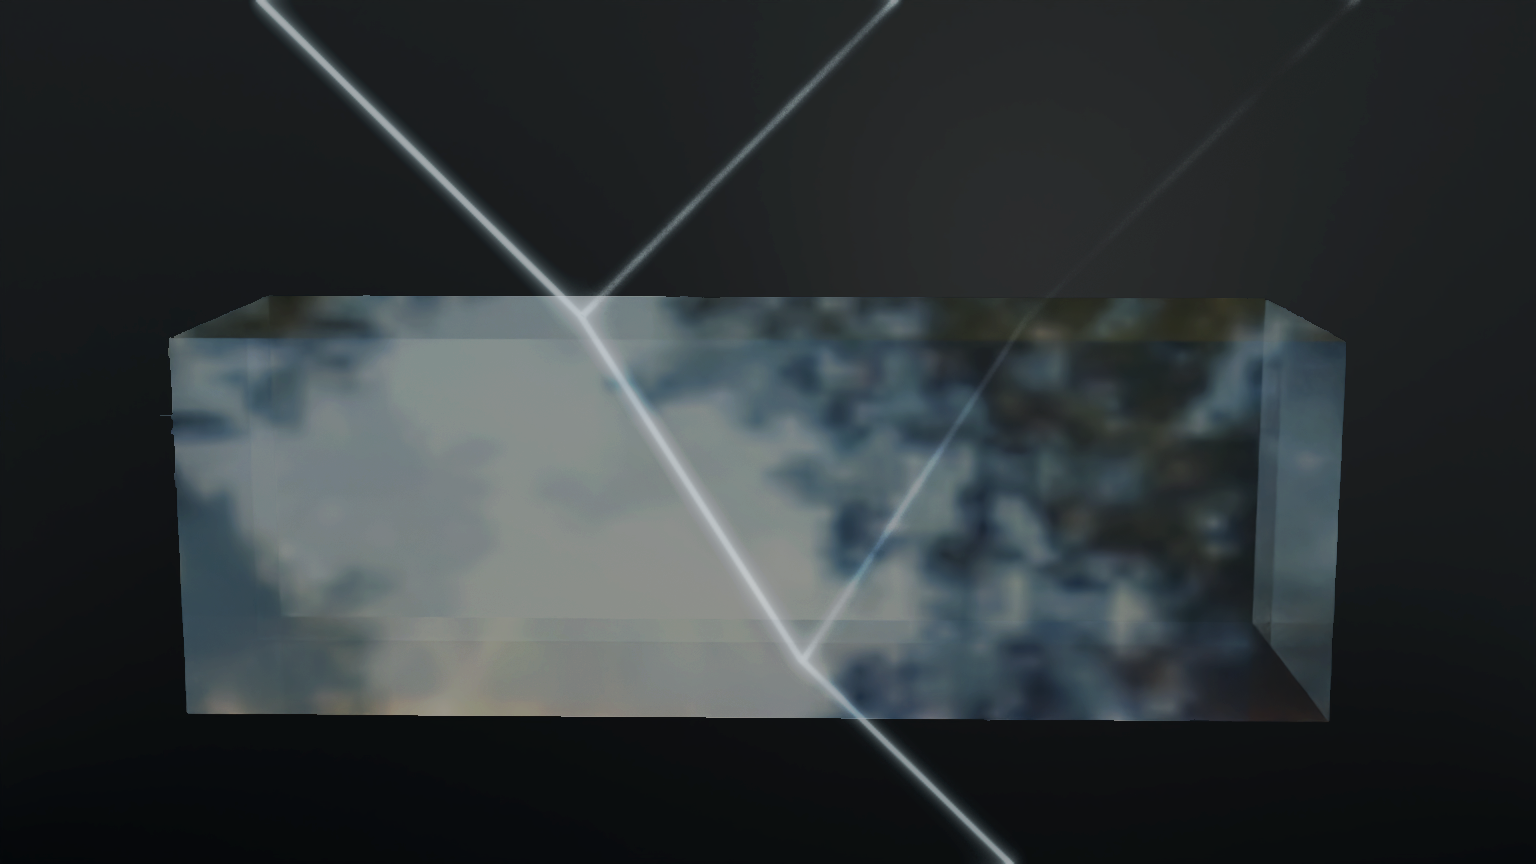
\includegraphics[width=0.90\linewidth]{luz_materia.png}
    \caption{Un raig de llum passa de l’aire a un medi transparent, com el vidre, la major part entra i canvia una mica de direcció: això és la refracció. Una petita part de la llum es reflecteix. A l’interior, quan la llum torna a arribar a una superfície, el procés es pot repetir i es produeixen diverses reflexions internes. Imatge creada per l’autor, CC BY 4.0.}
\end{figure}
El raig de llum que arriba a la superfície de separació entre dos materials s’anomena \textbf{raig incident}.

Una part de la llum pot rebotar: és la \textbf{reflexió}.

Si el segon material és transparent, una altra part pot entrar-hi. En fer-ho, normalment canvia de direcció: és la \textbf{refracció}.
\subsection{I llavors, què passa amb la fibra òptica?}

A la pràctica de classe hem vist que, dins d’una fibra òptica, la llum sembla seguir una corba. Així que alguna cosa està passant i ho hem d’investigar: fins i tot hem arribat a fer un nus de llum.

\begin{figure}[H]
    \centering
    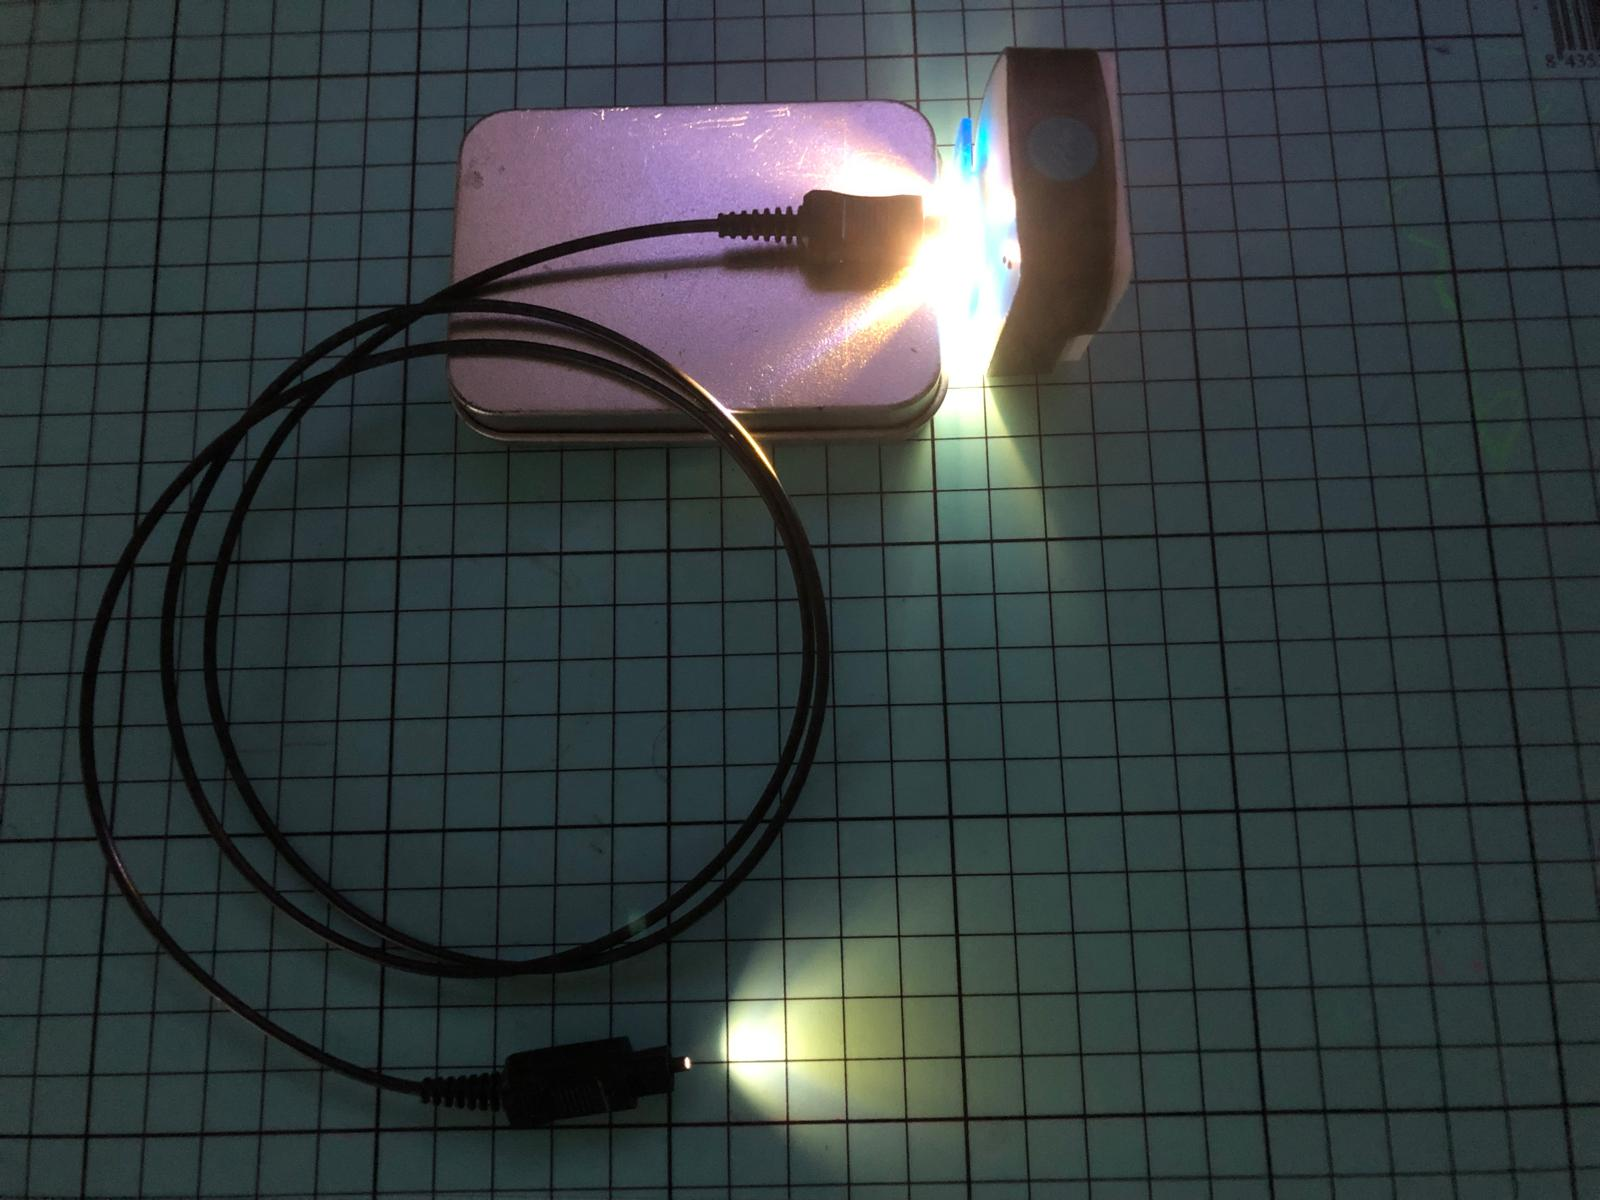
\includegraphics[width=0.7\linewidth]{fibra_optica_exp.jpg}
    \caption{En l’experiència que vam fer a classe, la llum que sortia de la llanterna semblava recórrer una corba dins de la fibra òptica. Tenim un cas entre mans: toca investigar què està passant.
. Imatge creada per l’autor, CC BY 4.0.}
\end{figure}

La fibra òptica està construïda perquè la llum quedi atrapada a l’interior. Quan arriba a les parets amb l’angle adequat, en lloc d’escapar-se, rebota completament cap a dins. Aquest fenomen s’anomena \textbf{reflexió interna total}.


\begin{figure}[H]
    \centering
    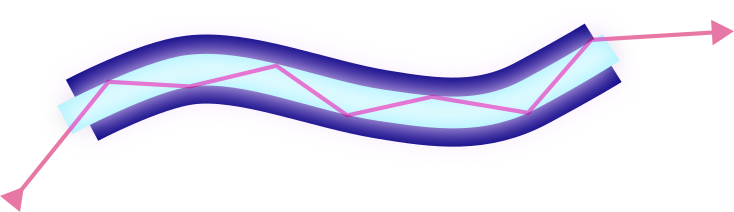
\includegraphics[width=1\linewidth]{fibra_optica.png}
    \caption{Dins de la fibra óptica, la llum continua fent petits trams rectes i rebotant dins de la fibra. Vista des de fora sembla que segueixi la seva forma, però no s’ha convertit de sobte en una serp.
. Imatge creada per l’autor, CC BY 4.0.}
\end{figure}

\subsection{Altres coses que fa la llum}

Si la llum arriba a un material que no és transparent, una part es pot reflectir i una altra pot ser absorbida.

Quan la llum és absorbida, la seva energia no desapareix. Normalment acaba transformant-se en energia interna del material, és a dir, contribueix a escalfar-lo. Per això una superfície negra al Sol acostuma a escalfar-se més que una de blanca.

En un metall ben polit es pot reflectir una gran part de la llum, com passa en un mirall.

\begin{figure}[H]
    \centering
    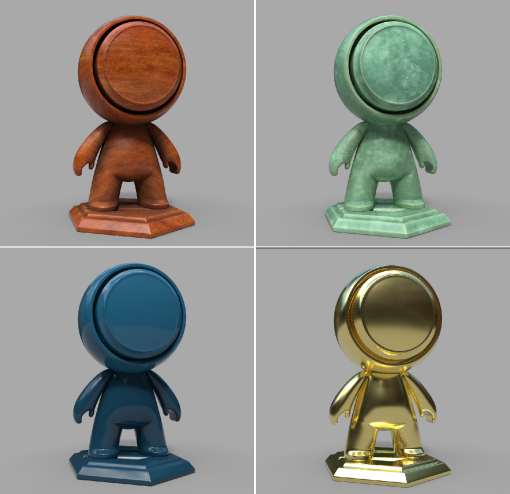
\includegraphics[width=1\linewidth]{materiales.png}
    \caption{Coneixent com es comporta la llum i sent capaços de descriure-la físicament, els artistes poden reproduir materials a l’ordinador amb un nivell de realisme impressionant. En aquesta imatge, creada amb el programari Substance Painter, veiem un mateix model amb materials molt diferents: fusta, pedra, plàstic i metall. El secret és simular com cada superfície reflecteix, absorbeix i dispersa la llum.
. Imatge creada per l’autor, CC BY 4.0.}
\end{figure}


\subsection{El misteri de l’armilla reflectant}

Les bandes reflectants d’una armilla poden contenir milers de petites estructures transparents, com ara microesferes de vidre.

\begin{figure}[H]
    \centering
    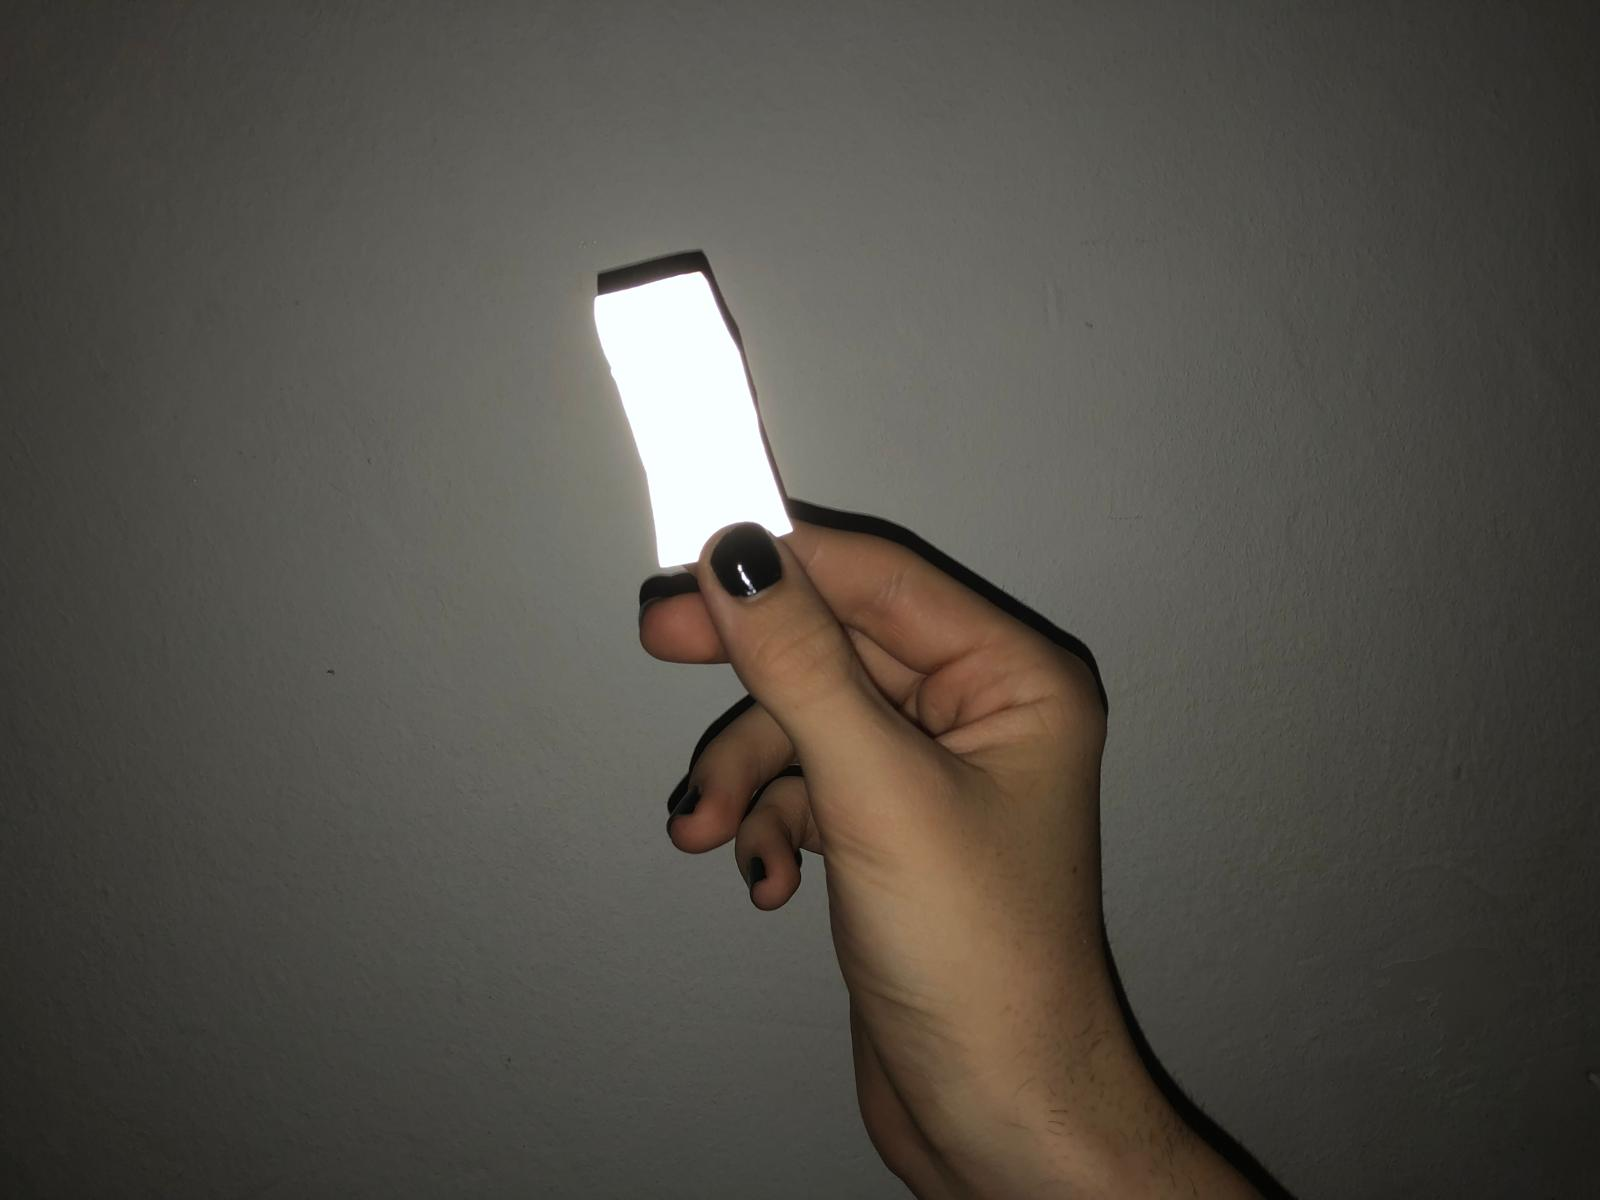
\includegraphics[width=0.7\linewidth]{tejido_reflectante_exp.jpg}
    \caption{Quan apuntem al teixit reflectant des d’una font de llum, com ara la càmera del mòbil amb la llanterna encesa o els fars d’un cotxe, ens retorna gairebé tota la llum que li enviem.
. Imatge creada per l’autor, CC BY 4.0.}
\end{figure}

Quan els fars d’un cotxe les il·luminen, la llum fa un petit viatge. Primer entra dins de la microesfera i es refracta. Després arriba a la part posterior, on es reflecteix. Finalment torna a travessar la microesfera i surt aproximadament en la direcció d’on havia vingut.
Això s’anomena \textbf{retroreflexió}: bona part de la llum torna cap a la font que l’ha enviat.

Per això, des del cotxe, les bandes semblen brillar tant. No estan produint aquella llum: te l’estan tornant.

A més, les parts de color groc o taronja intens de moltes armilles són fluorescents. Absorbeixen part de la radiació ultraviolada i la reemeten com a llum visible. No és màgia, encara que el resultat tingui certa tendència a semblar-ho.

\begin{figure}[H]
    \centering
    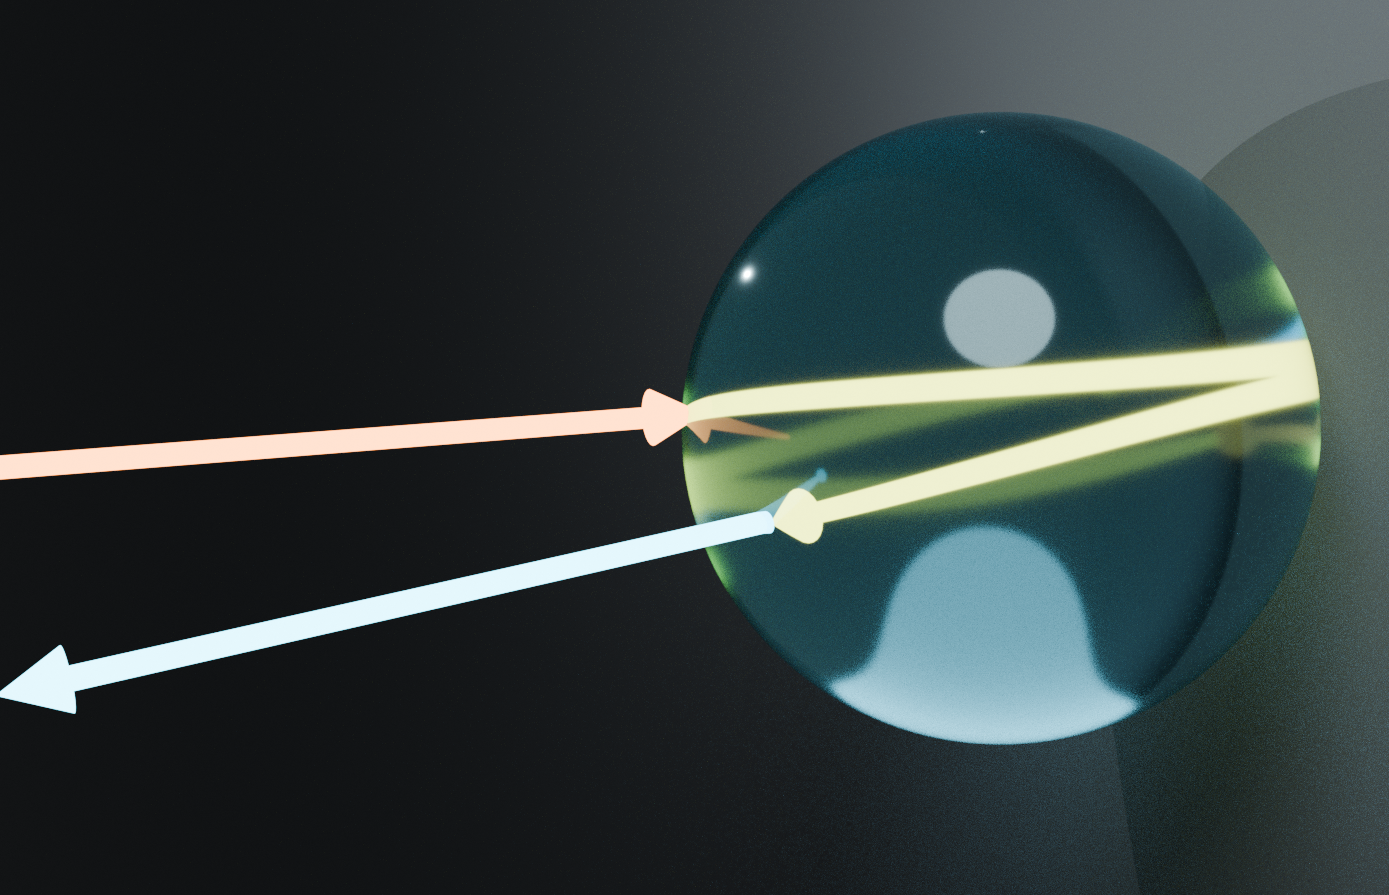
\includegraphics[width=1\linewidth]{microesfera.png}
    \caption{ Reproducció del recorregut de la llum dins d’una microesfera reflectant d’una armilla. Segueix el camí del raig incident, el raig refractat, el raig que rebota a la superfície reflectant i, finalment, el raig que surt gairebé en la mateixa direcció d’on havia arribat.
. Imatge creada per l’autor, CC BY 4.0.}
\end{figure}



\subsection{Ens fiquem una mica en la fotònica}

Hi ha una pila de components que treballen amb llum. Les cèl·lules solars transformen energia de la llum en energia elèctrica. Els LED fan pràcticament el camí contrari: utilitzen energia elèctrica per produir llum.
També existeixen sensors sensibles a la llum. Un fototransistor, per exemple, pot controlar el pas de corrent segons la quantitat de llum que rep.
Els cristalls líquids també poden canviar les seves propietats òptiques, enfosquint-se, quan hi apliquem electricitat.

Si combines aquestes coses com toca, pots construir aparells força interessants. Una careta de soldadura automàtica, per exemple, detecta la llum intensíssima de l’arc de soldadura i enfosqueix el visor gairebé immediatament.

\begin{figure}[H]
    \centering
    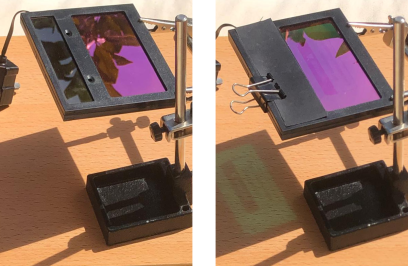
\includegraphics[width=1\linewidth]{soldador.png}
    \caption{ Quan el sensor de les ulleres de soldador queda exposat directament al Sol, el filtre de cristall líquid s’enfosqueix i bloqueja bona part de la llum. Si tapem el sensor amb una cartolina, el filtre deixa d’activar-se i torna a deixar passar la llum; això es pot veure a la zona verda de la part inferior.
 Imatge creada per l’autor, CC BY 4.0.}
\end{figure}



I això està bé, perquè mirar directament un arc de soldadura és una manera bastant estúpida de comprovar que la llum també pot ser perillosa.

\section{Nivell II }

\subsection{Índex de refracció}

La llum no viatja igual de ràpid en tots els medis. En el buit arriba a la seva velocitat màxima, aproximadament:

$$
c = 300\,000\ \text{km/s}
$$

\(c\) és el símbol que s’utilitza en física per representar, amb una sola lletra, la velocitat de la llum.. Per comparar els materials utilitzem una propietat anomenada \textbf{índex de refracció}:

$$
n=\frac{c}{v}
$$

on, com havíem dit, \(c\) és el símbol que s’utilitza en física per representar la velocitat de la llum en el buit, i \(v\) és la velocitat de la llum dins del material.
Alguns valors aproximats són:

\begin{center}
\begin{tabular}{lc}
Buit & 1,00\\
Aire & 1,0003\\
Aigua & 1,33\\
Vidre & 1,5\\
Diamant & 2,42
\end{tabular}
\end{center}

Com més gran és l’índex de refracció, més lentament es propaga la llum dins del material. Això també ens ajuda a entendre per què la llum canvia de direcció quan passa d’un material a un altre.

Si entra en un medi amb un índex de refracció més gran, el raig es desvia cap a la \textbf{normal}, que és simplement una línia imaginària perpendicular a la superfície.

Si passa cap a un medi amb un índex menor, es desvia en sentit contrari.

No cal complicar-ho gaire més de moment: el que ens interessa és veure que la desviació no és arbitrària. Depèn dels dos materials i de l’angle amb què arriba la llum.

\subsection{Reflexió i reflexió interna total}

En una reflexió normal hi ha una regla molt senzilla:

$$
\text{angle d’incidència}=\text{angle de reflexió}
$$

Si el raig arriba amb un angle de \(45^\circ\), surt amb \(45^\circ\) cap a l’altre costat de la normal. És una sort. Si els miralls decidissin cada vegada cap a on volen enviar la llum, arreglar-se els cabells seria un problema d’enginyeria.

En la refracció la situació és diferent: l’angle sí que canvia segons els materials. 

En física és molt habitual utilitzar les lletres de l’alfabet grec per representar angles. Les lletres i els seus noms els podeu trobar a la taula següent.

\begin{center}
\begin{tabular}{cc}
\textbf{Lletra grega} & \textbf{Nom} \\
\hline
$\alpha$ & alfa \\
$\beta$ & beta \\
$\gamma$ & gamma \\
\end{tabular}
\end{center}


\begin{figure}[H]
    \centering
    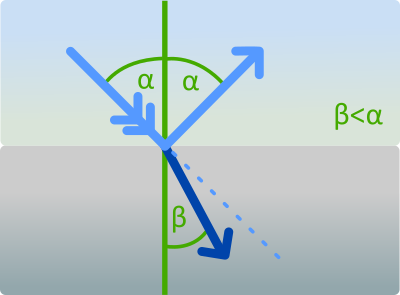
\includegraphics[width=0.6\linewidth]{aire_agua.png}
    \caption{ Quan el raig de llum passa de l’aire a l’aigua, disminueix la seva velocitat i canvia de direcció: es desvia cap a la normal. Per això l’angle de refracció \(\beta\) és més petit que l’angle d’incidència \(\alpha\).
La línia verda és la \textbf{normal}: una línia imaginària perpendicular a la superfície de separació entre els dos medis en el punt on arriba el raig. Els angles \(\alpha\) i \(\beta\) es mesuren sempre respecte d’aquesta línia.
 Imatge creada per l’autor, CC BY 4.0.}
\end{figure}


\begin{figure}[H]
    \centering
    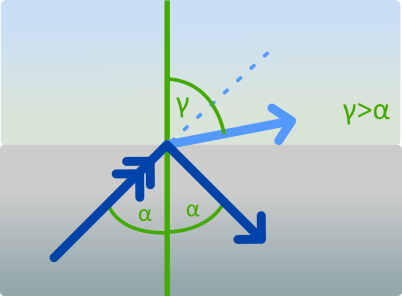
\includegraphics[width=0.6\linewidth]{agua_aire.png}
    \caption{ Quan la llum passa de l’aigua a l’aire, augmenta la seva velocitat i es desvia allunyant-se de la normal. Per això l’angle de refracció \(\gamma\) és més gran que l’angle d’incidència \(\alpha\).
La línia verda torna a ser la \textbf{normal}, perpendicular a la superfície de separació entre l’aigua i l’aire.
 Imatge creada per l’autor, CC BY 4.0.}
\end{figure}


\begin{figure}[H]
    \centering
    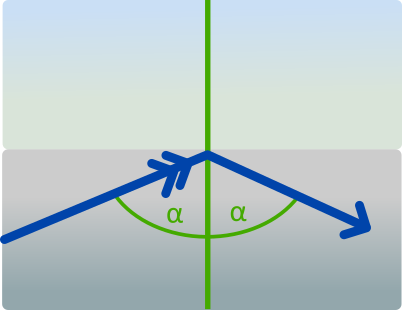
\includegraphics[width=0.6\linewidth]{reflexion_total.png}
    \caption{ Quan la llum intenta passar d’un medi amb un índex de refracció més gran cap a un altre de més petit, arriba un moment en què l’angle és tan gran que ja no aconsegueix sortir. Tota la llum es reflecteix cap a dins. Això és la \textbf{reflexió interna total}, i és exactament el que aprofita una fibra òptica per transportar llum a grans distàncies.
 Imatge creada per l’autor, CC BY 4.0.}
\end{figure}

\subsection{Metalls, plàstics i coses que brillen}

No només els metalls reflecteixen la llum. Un plàstic brillant, un vidre o la superfície de l’aigua també poden produir reflexos intensos, tot i que el mecanisme no és exactament el mateix que en un metall.

\begin{figure}[H]
    \centering
    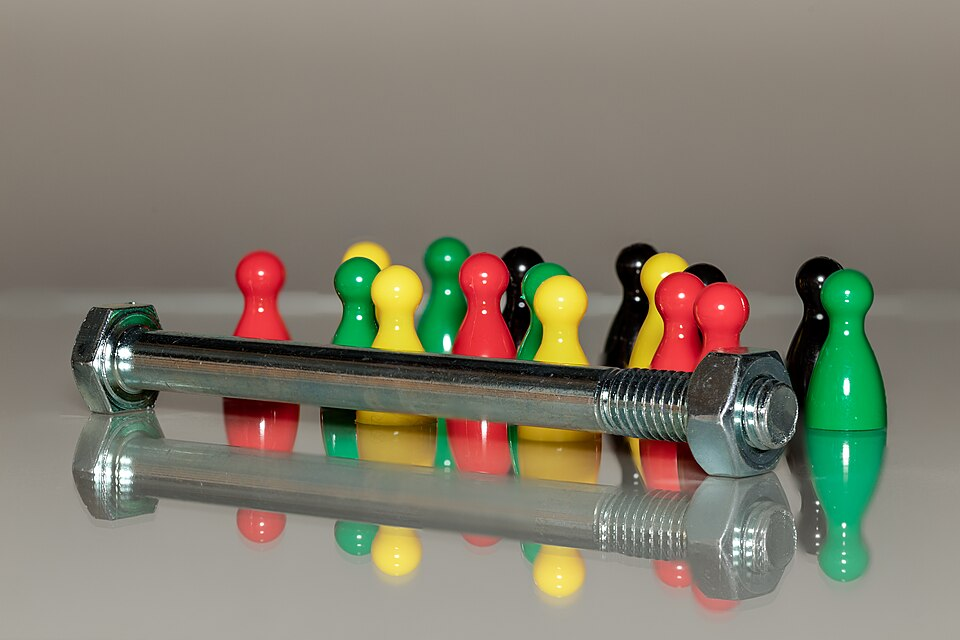
\includegraphics[width=0.8\linewidth]{Spielfiguren_mit_Schraube,_Titel__Beschränkt__--_2020_--_3851-7.jpg}
    \caption{ Llum reflectida en plàstic i en metall. Observa que no es comporta exactament igual: la llum també té les seves preferències.
 Imatge Dietmar Rabich, Wikimedia CC BY 4.0.}
\end{figure}


Els materials com el vidre o el plàstic són \textbf{dielèctrics}. Normalment deixen passar una part de la llum i en reflecteixen una altra.
Per això en una finestra pots veure alhora el carrer i una mica del teu propi reflex.





En alguns materials la cosa encara es complica més. La pell, una fulla o la cera permeten que part de la llum entri, reboti i es dispersi per l’interior abans de tornar a sortir.
A escala microscòpica, la llum està trobant estructures diferents contínuament i canviant de direcció moltes vegades.
El resultat és aquell aspecte una mica translúcid que veiem quan posem una mà davant d’una llanterna o una fulla davant del Sol.

\begin{figure}[H]
    \centering
    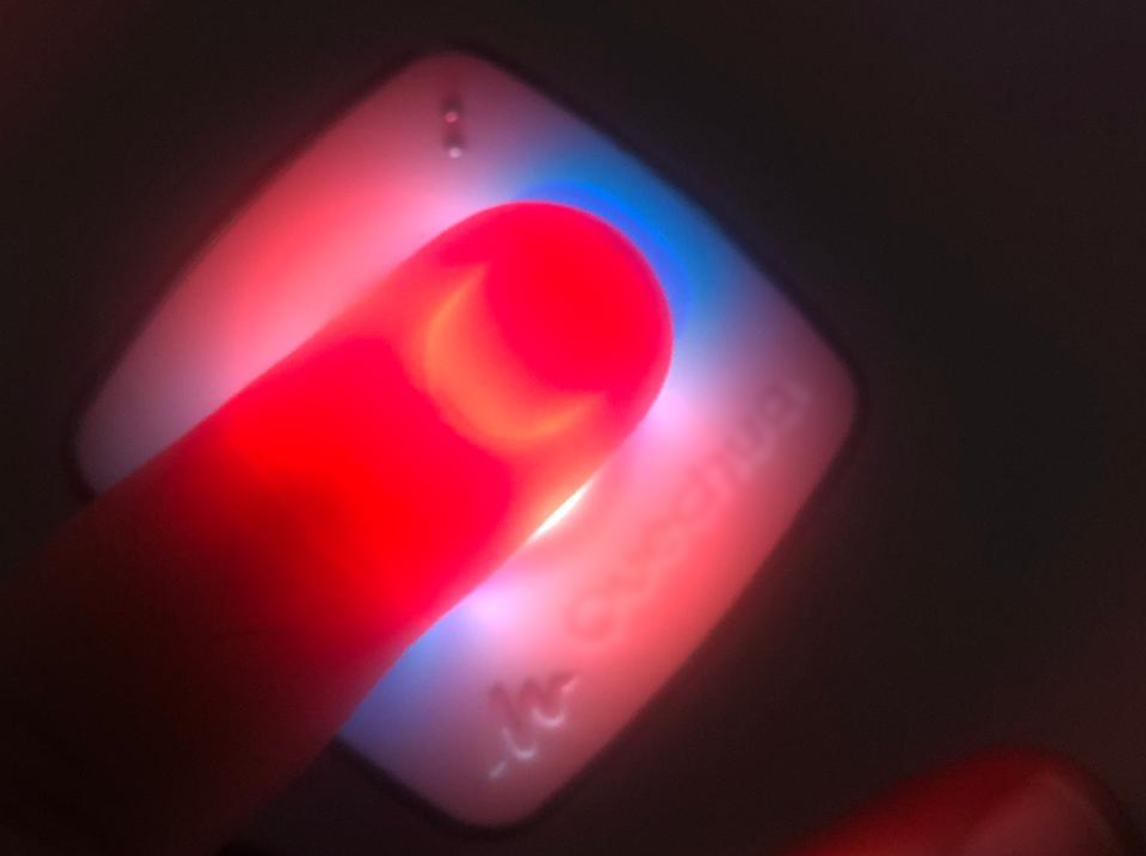
\includegraphics[width=0.8\linewidth]{dedo.41.png}
    \caption{ La llum de la llanterna travessa parcialment el dit. Els teixits n’absorbeixen una part i en deixen passar una altra. Com que la llum vermella travessa millor el dit que altres colors, el veiem il·luminat d’un vermell intens.
. Imatge creada per l’autor, CC BY 4.0.}
\end{figure}

Aquí ja comencem a veure una cosa important: dir simplement que un material és «transparent», «reflectant» o «opac» va bé per començar, però la realitat acostuma a tenir bastants més botons.



